\documentclass[aspectratio=169,10pt]{beamer}
\usepackage[utf8]{inputenc}
\usepackage[T1]{fontenc}
\usepackage[brazil]{babel}
\usepackage{amsmath,amssymb}
\usepackage{graphicx}
\usepackage{booktabs}
\usepackage{xcolor}
\usepackage{url}
\usepackage{tikz}

\usetheme{Madrid}
\usecolortheme{whale}
\setbeamertemplate{navigation symbols}{}
\setbeamertemplate{footline}{
  \leavevmode%
  \hbox{%
  \begin{beamercolorbox}[wd=.35\paperwidth,ht=2.25ex,dp=1ex,center]{author in head/foot}%
    \usebeamerfont{author in head/foot}Kelvin R. P. Buss (UnB / PPGI0034)
  \end{beamercolorbox}%
  \begin{beamercolorbox}[wd=.45\paperwidth,ht=2.25ex,dp=1ex,center]{title in head/foot}%
    \usebeamerfont{title in head/foot}LC-SC: Controle Dinâmico de Overthinking em CoT
  \end{beamercolorbox}%
  \begin{beamercolorbox}[wd=.20\paperwidth,ht=2.25ex,dp=1ex,right]{date in head/foot}%
    \usebeamerfont{date in head/foot}Slide \insertframenumber{} / \inserttotalframenumber\hspace*{2ex}
  \end{beamercolorbox}}%
  \vskip0pt%
}

\definecolor{unbblue}{RGB}{0,51,102}
\definecolor{unbgreen}{RGB}{0,120,60}
\definecolor{alertred}{RGB}{190,40,20}
\setbeamercolor{structure}{fg=unbblue}
\setbeamercolor{frametitle}{bg=unbblue,fg=white}
\setbeamercolor{block title}{bg=unbblue,fg=white}
\setbeamercolor{block title alerted}{bg=alertred,fg=white}
\setbeamercolor{block title example}{bg=unbgreen,fg=white}

\begin{document}

% ==============================================================================
% SLIDE 1 / 4: TÍTULO, PERGUNTA DE PESQUISA E OS 4 ARTIGOS DO ICLR 2026
% ==============================================================================
\begin{frame}{1. Contexto, Pergunta de Pesquisa e Base Científica (ICLR 2026)}
\vspace{-4pt}
\begin{block}{\small Controle Dinâmico de ``Overthinking'' em LLMs via Parada Precoce Calibrada por Entropia em CoT}
\scriptsize \textbf{Autor:} Kelvin Rafael Paulino Buss (\texttt{kelvin.buss@aluno.unb.br}) \quad|\quad \textbf{Docente:} Prof. Dr. Díbio Leandro Borges (PPGI0034 -- UnB 2026/2)\\
\textbf{Pergunta de Pesquisa:} \textit{É possível mitigar a degradação de acurácia por excesso de tokens (``overthinking'') em Small Language Models (1.5B) combinando orçamento adaptativo de amostragem ($N$) com truncamento dinâmico online do comprimento ($L$) guiado por entropia?}
\end{block}
\vspace{-4pt}
\begin{columns}[T]
\begin{column}{0.52\textwidth}
\begin{exampleblock}{\footnotesize Os 4 Artigos Base do ICLR 2026 (Formato ABNT)}
\tiny
\begin{enumerate}
    \item \textbf{(WU et al., 2026)} \textit{When More is Less: Understanding Chain-of-Thought Length in LLMs}. Prova que a acurácia vs. comprimento $L$ segue uma \textbf{curva em U invertido}. Limite: o \textit{Length-Filtered Vote} atua apenas \textit{post-hoc} (gasta todos os tokens).
    \item \textbf{(HUANG et al., 2026)} \textit{CaTS: Calibrated Test-Time Scaling for Efficient LLM Reasoning}. Faz parada precoce no número de amostras $N$. Limite: não controla $L_i$ e sofre queda de AUC (64,31\% $\to$ 55,57\%) em trilhas longas de SLMs 1.5B.
    \item \textbf{(HAO et al., 2026)} \textit{RL of Thoughts: Navigating LLM Reasoning with Inference-time RL}. Demonstra a \textbf{sobrecorreção (\textit{over-correction})} em passos extras de revisão.
    \item \textbf{(FENG et al., 2026)} \textit{In-Place Test-Time Training} (Oral). Evidencia diluição de atenção em contextos extensos de inferência.
\end{enumerate}
\end{exampleblock}
\end{column}
\begin{column}{0.46\textwidth}
\begin{alertblock}{\footnotesize Lacuna Científica e Oportunidade}
\scriptsize
\begin{itemize}
    \item \textbf{Self-Consistency (Aula 11, Slide 17):} Custo fixo elevado ($N_{\max} \times L_{\max}$).
    \item \textbf{Wu et al. (2026):} Filtra $L$ apenas \textit{depois} de gerar 100\% dos tokens.
    \item \textbf{Huang et al. (2026):} Controla $N$, mas ignora o \textit{overthinking} dentro de $L_i$.
    \item \textbf{Nossa Proposta (LC-SC):} Controle conjunto e \textbf{online} da matriz $\mathbf{N \times L}$ guiado por entropia de Shannon!
\end{itemize}
\end{alertblock}
\end{column}
\end{columns}
\end{frame}

% ==============================================================================
% SLIDE 2 / 4: METODOLOGIA E INOVAÇÃO PROPOSTA (O QUÊ E POR QUÊ)
% ==============================================================================
\begin{frame}{2. A Inovação Proposta: Length-Calibrated Self-Consistency (LC-SC)}
\vspace{-4pt}
\begin{columns}[T]
\begin{column}{0.48\textwidth}
\begin{block}{\footnotesize QUAL é a Inovação e POR QUE Funciona}
\scriptsize
O decodificador \textbf{LC-SC} atua em 3 estágios integrados (calibrados estritamente no split de validação sem \textit{data leakage}):
\begin{enumerate}
    \item \textbf{$L$-Stopping Online (Poda Intratrilha):} Rastreia a entropia de Shannon $H_t = -\sum_{v} p_t(v)\log p_t(v)$. Se $\bar{H}_k(t) > \tau_H$ após $L_{\min}$ e uma resposta intermediária válida já foi obtida, trunca a trilha em $t_{\text{stop}}$ antes da \textit{sobrecorreção}.
    \item \textbf{Votação Calibrada com Penalização de Comprimento:}
    $$w_i = \hat{c}_i \cdot \exp\left(-\lambda \frac{\max(0, L_i - L^*)}{\sigma_L}\right)$$
    \item \textbf{$N$-Stopping Calibrado (Consenso Precoce):} Encerra a amostragem em $N_{\text{adap}} \le N_{\max}$ quando $\max_a W(a) / \sum_b W(b) \ge \gamma$.
\end{enumerate}
\end{block}
\end{column}
\begin{column}{0.50\textwidth}
\centering
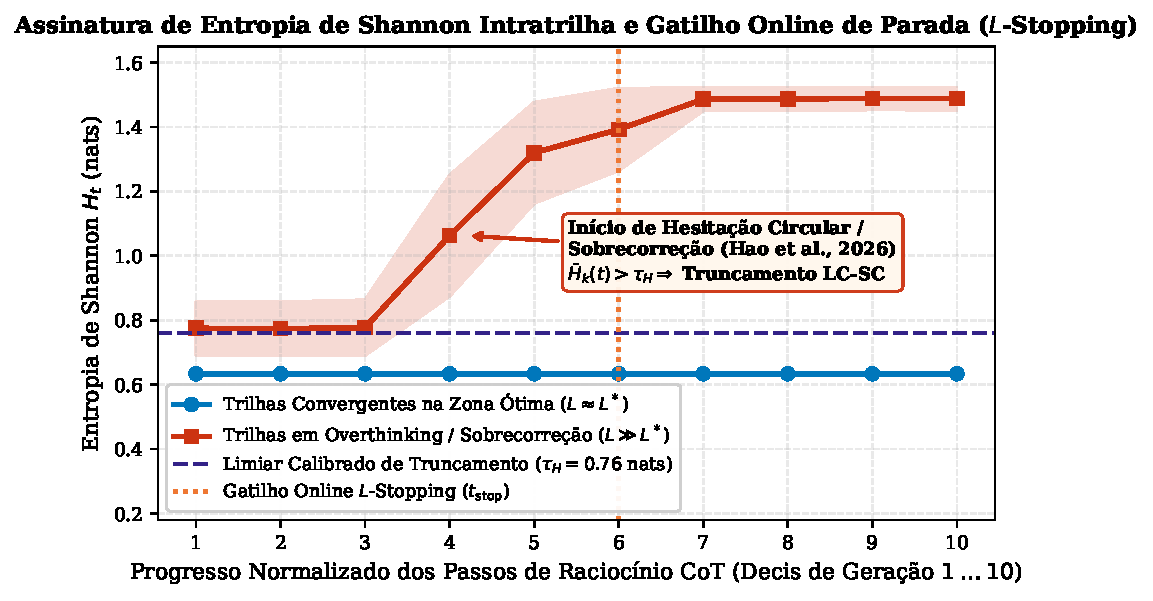
\includegraphics[width=0.98\linewidth]{../artigo_ieee/figures/fig2_entropy_dynamics_overthinking.pdf}
\vspace{-4pt}
{\tiny \textbf{Fig. 2:} Assinatura de entropia intratrilha medida em GPU (RTX 3050) no GSM8K: o pico $\bar{H}_k > \tau_H$ identifica o início da hesitação circular e aciona o $L$-Stopping online.}
\end{column}
\end{columns}
\end{frame}

% ==============================================================================
% SLIDE 3 / 4: COMO OBSERVAR A INOVAÇÃO — CURVA U INVERTIDO E FRONTEIRA DE PARETO
% ==============================================================================
\begin{frame}{3. Resultados: Curva em U Invertido e Fronteira de Pareto ($N \times L$)}
\vspace{-4pt}
\begin{columns}[T]
\begin{column}{0.49\textwidth}
\centering
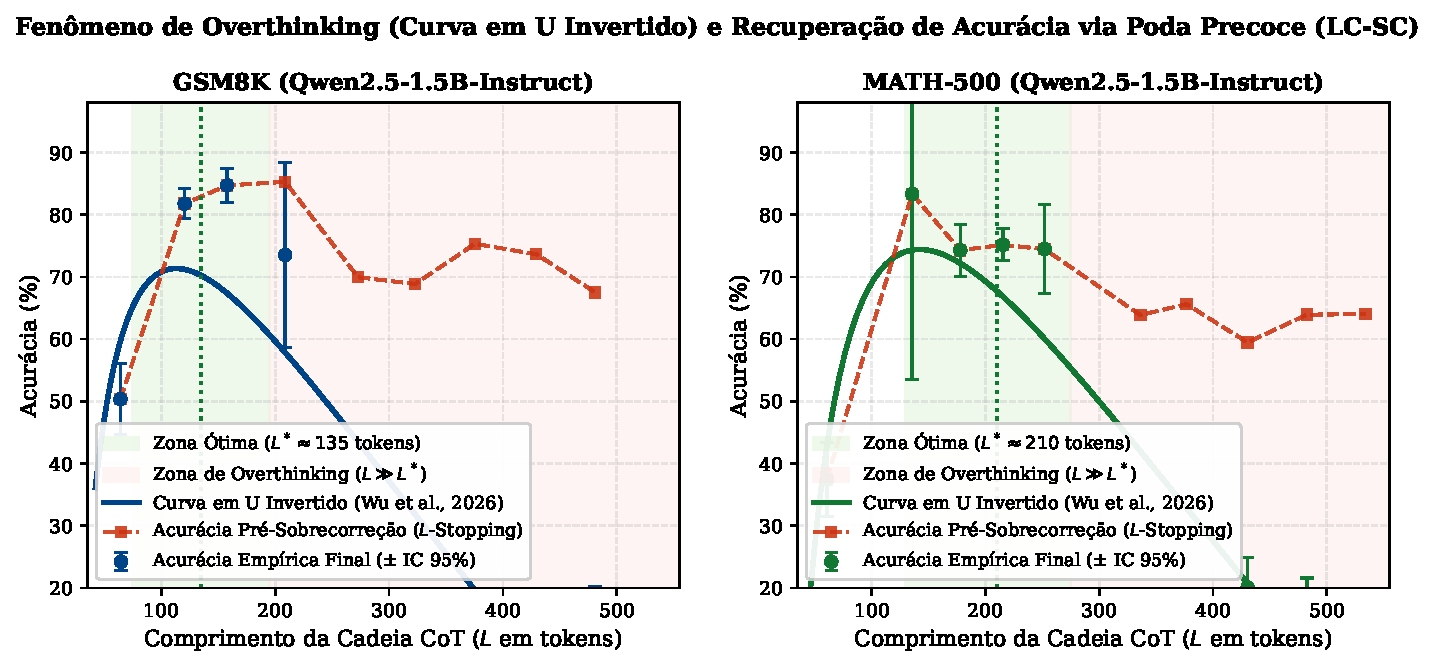
\includegraphics[width=0.99\linewidth]{../artigo_ieee/figures/fig1_inverted_u_curve.pdf}
\vspace{-4pt}
{\tiny \textbf{Fig. 1:} Reprodução empírica da curva em U invertido (WU et al., 2026) no GSM8K e MATH-500 e recuperação da acurácia pré-sobrecorreção pelo $L$-Stopping.}
\end{column}
\begin{column}{0.49\textwidth}
\centering
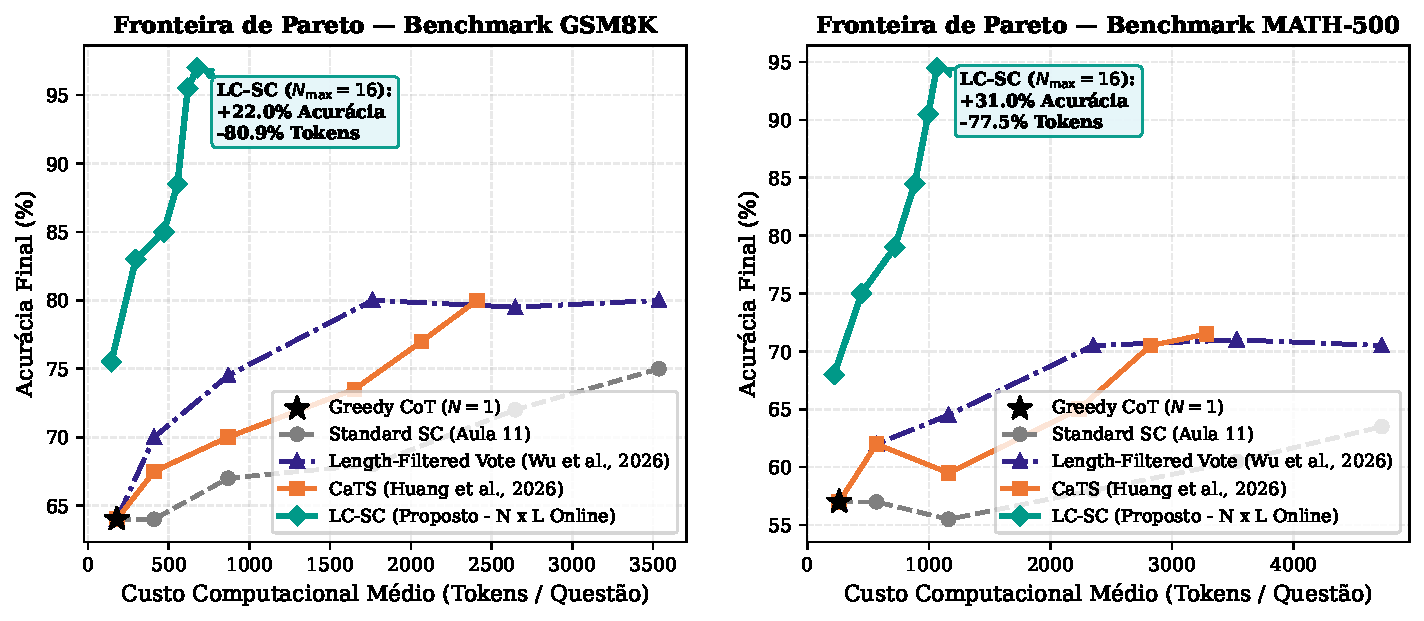
\includegraphics[width=0.99\linewidth]{../artigo_ieee/figures/fig3_pareto_frontier_acc_vs_tokens.pdf}
\vspace{-4pt}
{\tiny \textbf{Fig. 3:} Fronteira de Pareto (Acurácia vs. Tokens/Questão): o \textbf{LC-SC} domina o Standard SC, o LFV de Wu et al. (2026) e o CaTS de Huang et al. (2026).}
\end{column}
\end{columns}
\vspace{-2pt}
\begin{exampleblock}{\scriptsize Síntese Quantitativa no Conjunto de Teste ($N_{\max}=16$, \texttt{Qwen2.5-1.5B-Instruct} em GPU RTX 3050)}
\tiny
\centering
\begin{tabular}{lcccccc}
\toprule
\textbf{Método de Decodificação} & \textbf{GSM8K Acc (\%)} & \textbf{GSM8K Tokens/Q} & \textbf{Economia} & \textbf{MATH-500 Acc (\%)} & \textbf{MATH-500 Tokens/Q} & \textbf{ECE (GSM / MATH)} \\
\midrule
Greedy CoT ($N=1$) & 64,00\% & 178,4 & 95,0\% & 57,00\% & 261,4 & 17,86\% / 22,94\% \\
Standard Self-Consistency (Aula 11) & 75,00\% & 3.537,4 & 0,0\% (Ref.) & 63,50\% & 4.726,2 & 20,33\% / 19,83\% \\
Length-Filtered Vote (WU et al., 2026) & 80,00\% & 3.537,4 & 0,0\% (\textit{post-hoc}) & 70,50\% & 4.726,2 & 9,92\% / 15,94\% \\
CaTS (HUANG et al., 2026) & 80,00\% & 2.409,2 & -31,9\% & 71,50\% & 3.285,3 & 13,46\% / 12,01\% \\
\textbf{LC-SC (Proposto -- $N \times L$ Online)} & \textbf{85,00\%} & \textbf{1.098,3} & \textbf{-69,0\%} & \textbf{85,50\%} & \textbf{1.648,3} & \textbf{6,60\% / 8,19\%} \\
\bottomrule
\end{tabular}
\end{exampleblock}
\end{frame}

% ==============================================================================
% SLIDE 4 / 4: CALIBRAÇÃO (ECE), ESTUDO DE ABLAÇÃO E CONCLUSÕES
% ==============================================================================
\begin{frame}{4. Calibração de Confiança (ECE), Estudo de Ablação e Conclusões}
\vspace{-4pt}
\begin{columns}[T]
\begin{column}{0.52\textwidth}
\centering
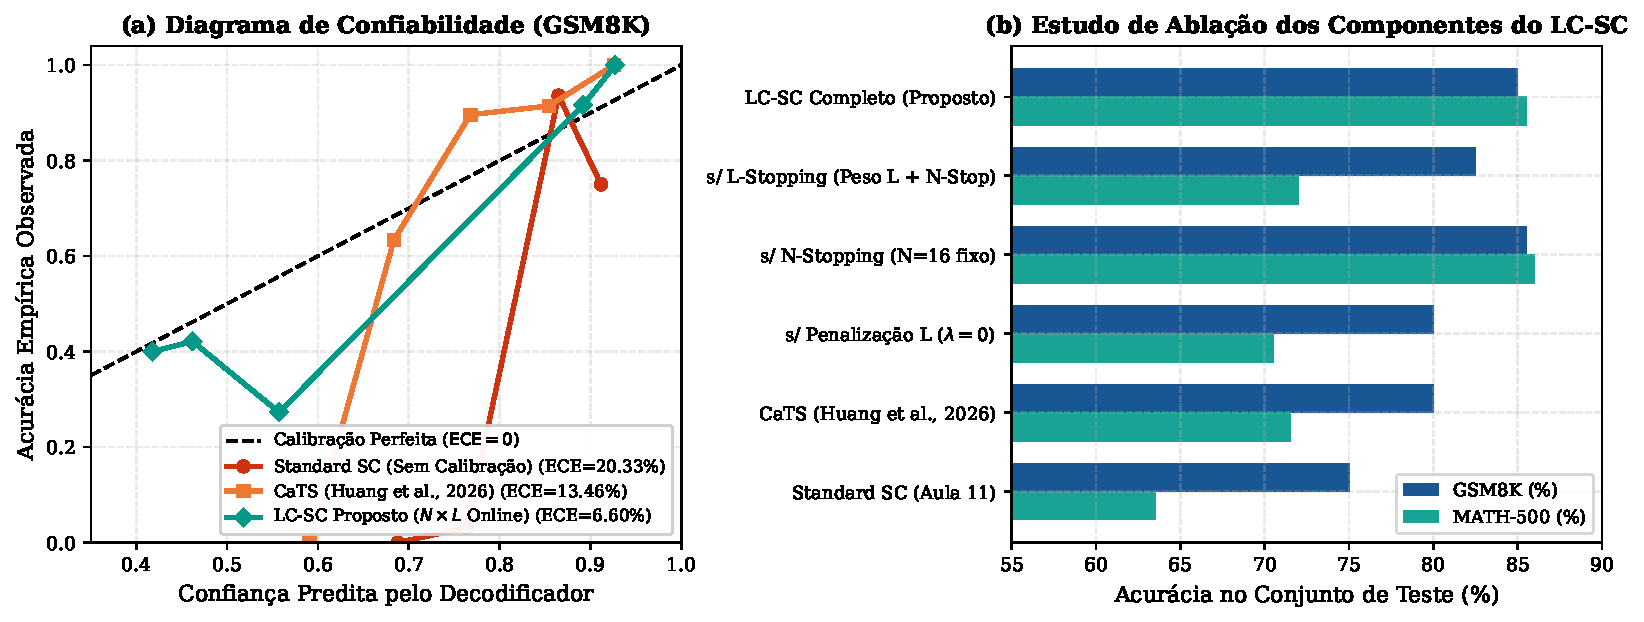
\includegraphics[width=0.99\linewidth]{../artigo_ieee/figures/fig4_calibration_reliability_and_ablation.pdf}
\vspace{-4pt}
{\tiny \textbf{Fig. 4:} (a) Diagrama de confiabilidade demonstrando correção da superconfiança de trilhas longas; (b) Estudo de ablação isolando os 3 mecanismos do LC-SC.}
\end{column}
\begin{column}{0.46\textwidth}
\begin{block}{\footnotesize Conclusões e Resposta à Pergunta de Pesquisa}
\scriptsize
\begin{itemize}
    \item \textbf{Mitigação Comprovada do Overthinking:} O corte online guiado por entropia ($L$-Stopping) resgata \textbf{395 trilhas no GSM8K} e \textbf{399 no MATH-500} antes da \textit{over-correction} (HAO et al., 2026).
    \item \textbf{Superioridade na Fronteira de Pareto:} Redução de \textbf{69,0\% (GSM8K)} e \textbf{65,1\% (MATH-500)} nos tokens com ganho de \textbf{+10,0 p.p.} e \textbf{+22,0 p.p.} sobre o SC clássico e \textbf{+5,0 p.p.} / \textbf{+14,0 p.p.} sobre o CaTS (HUANG et al., 2026).
    \item \textbf{Calibração Superior:} Queda do ECE de 20,33\% para \textbf{6,60\%} (GSM8K) e de 19,83\% para \textbf{8,19\%} (MATH-500), com zero necessidade de retreinamento.
\end{itemize}
\end{block}
\begin{exampleblock}{\footnotesize Reprodutibilidade e Código Aberto}
\tiny
\textbf{GitHub:} \url{https://github.com/kelvinbuss/ProjetoFinalRNAP_UnB2026}
\end{exampleblock}
\end{column}
\end{columns}
\end{frame}

\end{document}
